
%(BEGIN_QUESTION)
% Copyright 2007, Tony R. Kuphaldt, released under the Creative Commons Attribution License (v 1.0)
% This means you may do almost anything with this work of mine, so long as you give me proper credit

A student, weary of performing ``thought experiments,'' decides to perform a {\it real} experiment to better understand phase changes.  She assembles a primitive steam boiler using a pressure cooker, a pressure gauge, a thermometer, a couple of valves, and a burner as a source of heat:

$$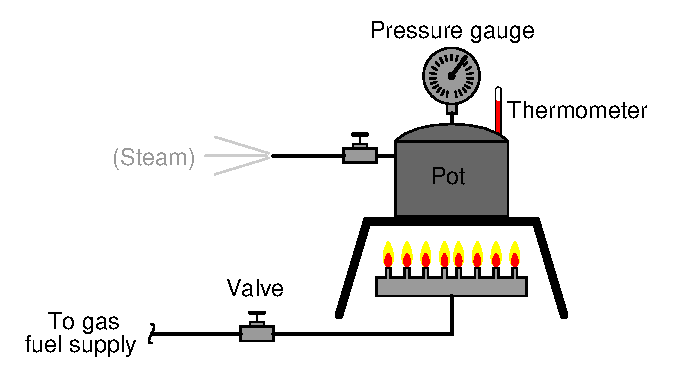
\includegraphics[width=15.5cm]{i01795x01.eps}$$

Her hypothesis is that boiler temperature may be controlled by fuel gas flow (burner heat rate output), and that boiler pressure may be controlled by steam flow out of the boiler.  Two process measurements, and two control valves: what could be simpler?

However, the student soon discovers that she cannot {\it independently} control boiler pressure and boiler temperature.  When fuel flow is increased, {\it both} pressure and temperature rise; as the steam valve is opened, {\it both} pressure and temperature decrease.

\vskip 10pt

Explain why this experiment did not go as planned, and what important lesson this student should learn about phase changes.

\underbar{file i01795}
%(END_QUESTION)





%(BEGIN_ANSWER)

The {\it saturated vapor pressure} of a substance is a direct function of temperature.  If we increase the heat rate so as to boil water faster, we will build up more pressure in the vessel, causing the boiling point to rise.  Continued heat flow into the water from the burner will then cause the temperature to rise to match the rising boiling point.

If we try to vent more steam, we cause the pressure in the vessel to decrease.  More water begins to boil, which removes heat energy from the water, causing its temperature to drop.

\vskip 10pt

A sophisticated way of stating the problem is that the student assumed {\it two degrees of freedom} in this process, where there in fact is only one degree of freedom.

%(END_ANSWER)





%(BEGIN_NOTES)


%INDEX% Physics, heat and temperature: saturated steam pressure versus temperature

%(END_NOTES)


